

%% AP Physics MC Questions Archive
%%----------------------------------------


%% One Dimensional Motion with Graphs
%%----------------------------------------
\newcommand{\apMotionGraphsQOne}{
\begin{tikzpicture}
    \begin{axis}[
        axis y line=left,
        axis x line=bottom,
        axis line style={->},
        xlabel={time},
        xtick=\empty,
        ylabel={position},
        ytick=\empty,
        xmin=0,xmax=11,
        ymin=0,ymax=11,
        width=0.8\columnwidth,
        height=0.5\columnwidth,
    ]
    \addplot[mark=\empty,thick,smooth] plot coordinates { (0,3) (5,9) (8,1) (10,6) };
    %% guesswork
    \draw[fill] (axis cs:1,4.5) circle (1.5pt) node[anchor=north] {$A$};
    \draw[fill] (axis cs:3,7.3) circle (1.5pt) node[anchor=north] {$B$};
    \draw[fill] (axis cs:5,9) circle (1.5pt) node[anchor=north] {$C$};
    \draw[fill] (axis cs:6.7,5) circle (1.5pt) node[anchor=west] {$D$};
    \draw[fill] (axis cs:8,1) circle (1.5pt) node[anchor=south] {$E$};
    \end{axis}
\end{tikzpicture}
}

\element{ap}{
\begin{question}{1d-motion-graphs-q01}
    %Base your answers to questions 1 through 3 on
    The position versus time graph below shows the motion of a particle on a straight line.
    \begin{center}
        \apMotionGraphsQOne
    \end{center}
    At which of the labeled points is the magnitude of the velocity greatest?
    \begin{multicols}{5}
    \begin{choices}[o]
        \wrongchoice{$A$}
        \wrongchoice{$B$}
        \wrongchoice{$C$}
      \correctchoice{$D$}
        \wrongchoice{$E$}
    \end{choices}
    \end{multicols}
\end{question}
}

\element{ap}{
\begin{question}{1d-motion-graphs-q02}
    %Base your answers to questions 1 through 3 on
    The position versus time graph below shows the motion of a particle on a straight line.
    \begin{center}
        \apMotionGraphsQOne
    \end{center}
    At which of the labeled points is the velocity zero?
    \begin{multicols}{3}
    \begin{choices}
        \wrongchoice{$B$ only}
        \wrongchoice{$E$ only}
        \wrongchoice{$D$ only}
        \wrongchoice{$C$ and $D$}
      \correctchoice{$C$ and $E$}
    \end{choices}
    \end{multicols}
\end{question}
}

\element{ap}{
\begin{question}{1d-motion-graphs-q03}
    %Base your answers to questions 1 through 3 on
    The position versus time graph below shows the motion of a particle on a straight line.
    \begin{center}
        \apMotionGraphsQOne
    \end{center}
    At which of the labeled points is the magnitude of the acceleration greatest?
    \begin{multicols}{5}
    \begin{choices}[o]
        \wrongchoice{$A$}
        \wrongchoice{$B$}
        \wrongchoice{$C$}
        \wrongchoice{$D$}
      \correctchoice{$E$}
    \end{choices}
    \end{multicols}
\end{question}
}

\newcommand{\apMotionGraphsQFour}{
\begin{tikzpicture}
    \begin{axis}[
        axis y line=left,
        axis x line=middle,
        axis line style={->},
        xlabel={time},
        x unit=\si{\second},
        xtick={0,2,4,6,8,10,12,14},
        minor x tick num=1,
        ylabel={velocity},
        y unit=\si{\meter\per\second},
        ytick={-20,-10,0,10,20},
        minor y tick num=2,
        grid=major,
        xmin=0,xmax=14.5,
        ymin=-21,ymax=21,
        width=0.8\columnwidth,
        height=0.5\columnwidth,
    ]
    \addplot[line width=1pt,mark=\empty] plot coordinates {(0,0) (3,20) (7,-20) (10,-20) (11,0) (14,0)};
    \end{axis}
\end{tikzpicture}
}

\element{ap}{
\begin{question}{1d-motion-graphs-q04}
    The velocity versus time graph below shows the motion of a particle on a straight line.
    \begin{center}
        \apMotionGraphsQFour
    \end{center}
    At what time after $t=0$ does the object again pass through its initial position?
    \begin{multicols}{3}
    \begin{choices}
        \wrongchoice{\SI{3}{\second}}
        \wrongchoice{\SI{5}{\second}}
        \wrongchoice{\SI{7}{\second}}
      \correctchoice{\SI{9}{\second}}
        \wrongchoice{\SI{10}{\second}}
    \end{choices}
    \end{multicols}
\end{question}
}

\element{ap}{
\begin{question}{1d-motion-graphs-q05}
    The velocity versus time graph below shows the motion of a particle on a straight line.
    \begin{center}
        \apMotionGraphsQFour
    \end{center}
    During which interval does the particle have the same average acceleration as $\SI{12}{\second}<t<\SI{14}{\second}$?
    \begin{multicols}{2}
    \begin{choices}
        \wrongchoice{$\SI{9}{\second}<t<\SI{11}{\second}$}
        \wrongchoice{$\SI{2}{\second}<t<\SI{5}{\second}$}
        \wrongchoice{$\SI{0}{\second}<t<\SI{3}{\second}$}
        \wrongchoice{$\SI{3}{\second}<t<\SI{7}{\second}$}
      \correctchoice{$\SI{5}{\second}<t<\SI{11}{\second}$}
    \end{choices}
    \end{multicols}
\end{question}
}

\newcommand{\apOneDMotionGraphsQSix}{
\begin{tikzpicture}
    \begin{axis}[
        axis y line=left,
        axis x line=bottom,
        axis line style={->},
        xlabel={time},
        xtick=\empty,
        ylabel={displacement},
        ytick=\empty,
        xmin=0,xmax=11,
        ymin=0,ymax=11,
        width=0.8\columnwidth,
        height=0.5\columnwidth,
    ]
    \addplot[line width=1pt,domain=0:10] {x};
    \end{axis}
\end{tikzpicture}
}

\element{ap}{
\begin{question}{1d-motion-graphs-q06}
    The displacement $x$ of an object moving in one dimension is shown below as a function of time $t$.
    \begin{center}
        \apOneDMotionGraphsQSix
    \end{center}
    The acceleration of this object must be:
    \begin{choices}
      \correctchoice{zero}
        \wrongchoice{constant and positive}
        \wrongchoice{constant and negative}
        \wrongchoice{increasing}
        \wrongchoice{decreasing}
    \end{choices}
\end{question}
}

\element{ap}{
\begin{question}{1d-motion-graphs-q07}
    The displacement of an object moving in one dimension is shown below as a function of time.
    \begin{center}
        \apOneDMotionGraphsQSix
    \end{center}
    The velocity of this object must be:
    \begin{choices}
        \wrongchoice{zero}
      \correctchoice{constant and positive}
        \wrongchoice{constant and negative}
        \wrongchoice{increasing}
        \wrongchoice{decreasing}
    \end{choices}
\end{question}
}

\element{ap}{
\begin{question}{1d-motion-graphs-q08}
    An object undergoes constant acceleration.
    Initially at rest, the object travels \SI{5}{\meter} in the first second.
    What additional distance will be covered in the next second?
    \begin{multicols}{3}
    \begin{choices}
        \wrongchoice{\SI{5}{\meter}}
        \wrongchoice{\SI{10}{\meter}}
      \correctchoice{\SI{15}{\meter}}
        \wrongchoice{\SI{20}{\meter}}
        \wrongchoice{\SI{25}{\meter}}
    \end{choices}
    \end{multicols}
\end{question}
}

\element{ap}{
\begin{question}{1d-motion-graphs-q09}
    A simple pendulum oscillates with amplitude $A$ and period $T$,
        as represented on the graph below.
    \begin{center}
    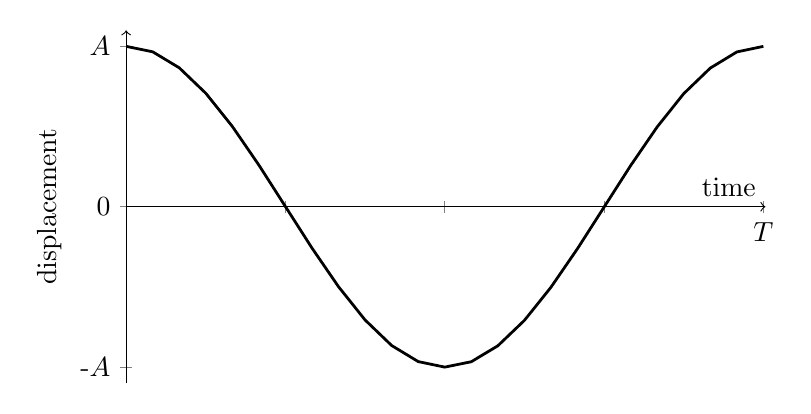
\begin{tikzpicture}
        \begin{axis}[
            axis y line=left,
            axis x line=middle,
            axis line style={->},
            xlabel={time},
            xtick={0,1.57,3.14,4.71,6.28},
            xticklabels={,,,,$T$},
            ylabel={displacement},
            ytick={-1,0,1},
            yticklabels={-$A$,0,$A$},
            xmin=0,xmax=6.30,
            ymin=-1.1,ymax=1.1,
            width=0.8\columnwidth,
            height=0.5\columnwidth,
        ]
        \addplot[line width=1pt,domain=0:6.28] {cos(deg(x))};
        \end{axis}
    \end{tikzpicture}
    \end{center}
    The nature of the velocity $v$ and acceleration $a$ of the object at time $\dfrac{T}{2}$ is best represented by which of the following?
    \begin{multicols}{2}
    \begin{choices}
        \wrongchoice{$v < 0$, $a < 0$}
        \wrongchoice{$v < 0$, $a = 0$}
        \wrongchoice{$v < 0$, $a > 0$}
      \correctchoice{$v = 0$, $a > 0$}
        \wrongchoice{$v = 0$, $a = 0$}
    \end{choices}
    \end{multicols}
\end{question}
}

\element{ap}{
\begin{question}{1d-motion-graphs-q10}
    The graph below represents the motion of an object traveling in a straight line as a function of time.
    \begin{center}
    \begin{tikzpicture}
        \begin{axis}[
            axis y line=left,
            axis x line=bottom,
            axis line style={->},
            xlabel={time},
            y unit=\si{\second},
            xtick={0,1,2,3,4,5},
            ylabel={displacement},
            y unit=\si{\meter},
            ytick={0,1,2},
            xmin=0,xmax=5.2,
            ymin=0,ymax=2.2,
            grid=major,
            width=0.8\columnwidth,
            height=0.5\columnwidth,
        ]
        \addplot[line width=1pt,mark=\empty] plot coordinates {(0,0) (2,2) (4,2) (5,1)};
        \end{axis}
    \end{tikzpicture}
    \end{center}
    What is the average speed of the object during the first four seconds?
    \begin{multicols}{3}
    \begin{choices}
        \wrongchoice{\SI{0}{\meter\per\second}}
        \wrongchoice{\SI{0.2}{\meter\per\second}}
      \correctchoice{\SI{0.5}{\meter\per\second}}
        \wrongchoice{\SI{1}{\meter\per\second}}
        \wrongchoice{\SI{2}{\meter\per\second}}
    \end{choices}
    \end{multicols}
\end{question}
}

\element{ap}{
\begin{question}{1d-motion-graphs-q11}
    Which pair of graphs represents the same one-dimensional motion?
    \begin{choices}
        \AMCboxDimensions{down=-2.5em}
        \wrongchoice{
            \begin{tikzpicture}
                \begin{groupplot}[
                        axis y line=left,
                        axis x line=bottom,
                        axis line style={->},
                        group style={group size=2 by 1},
                        xlabel={time},
                        xtick=\empty,
                        ytick=\empty,
                        xmin=0,xmax=11,
                        ymin=0,ymax=11,
                        width=0.45\columnwidth,
                    ]
                    \nextgroupplot[
                        ylabel={distance},
                    ] \addplot[line width=1pt,domain=0:10] {5};
                    \nextgroupplot[
                        ylabel={speed},
                    ] \addplot[line width=1pt,domain=0:10] {x};
                \end{groupplot}
            \end{tikzpicture}
        }
        \wrongchoice{
            \begin{tikzpicture}
                \begin{groupplot}[
                        axis y line=left,
                        axis x line=bottom,
                        axis line style={->},
                        group style={group size=2 by 1},
                        xlabel={time},
                        xtick=\empty,
                        ytick=\empty,
                        xmin=0,xmax=11,
                        ymin=0,ymax=11,
                        width=0.45\columnwidth,
                    ]
                    \nextgroupplot[
                        ylabel={distance},
                    ] \addplot[line width=1pt,domain=0:10] {10- 0.1*x*x};
                    \nextgroupplot[
                        ylabel={speed},
                    ] \addplot[line width=1pt,domain=0:10] {5};
                \end{groupplot}
            \end{tikzpicture}
        }
        %% ANS is C
        \correctchoice{
            \begin{tikzpicture}
                \begin{groupplot}[
                        axis y line=left,
                        axis x line=bottom,
                        axis line style={->},
                        group style={group size=2 by 1},
                        xlabel={time},
                        xtick=\empty,
                        ytick=\empty,
                        xmin=0,xmax=11,
                        ymin=0,ymax=11,
                        width=0.45\columnwidth,
                    ]
                    \nextgroupplot[
                        ylabel={distance},
                    ] \addplot[line width=1pt,domain=0:10] {0.1*x*x};
                    \nextgroupplot[
                        ylabel={speed},
                    ] \addplot[line width=1pt,domain=0:10] {x};
                \end{groupplot}
            \end{tikzpicture}
        }
        \wrongchoice{
            \begin{tikzpicture}
                \begin{groupplot}[
                        axis y line=left,
                        axis x line=bottom,
                        axis line style={->},
                        group style={group size=2 by 1},
                        xlabel={time},
                        xtick=\empty,
                        ytick=\empty,
                        xmin=0,xmax=11,
                        ymin=0,ymax=11,
                        width=0.45\columnwidth,
                    ]
                    \nextgroupplot[
                        ylabel={distance},
                    ] \addplot[line width=1pt,domain=0:10] {10-x};
                    \nextgroupplot[
                        ylabel={speed},
                    ] \addplot[line width=1pt,domain=0:10] {x};
                \end{groupplot}
            \end{tikzpicture}
        }
        %\wrongchoice{none of the provided}
    \end{choices}
\end{question}
}

\element{ap}{
\begin{questionmult}{1d-motion-graphs-q12}
    %Base your answer to the following question on the graphs below,
    %    which plot the velocity of a particle with respect to time.
    In which of these cases is the rate of change of the particle's displacement constant?
    \begin{multicols}{2}
    \begin{choices}
        \AMCboxDimensions{down=-2.5em}
        \wrongchoice{
            \begin{tikzpicture}
                \begin{axis}[
                    axis y line=left,
                    axis x line=bottom,
                    axis line style={->},
                    xlabel={time},
                    xtick=\empty,
                    ylabel={velocity},
                    ytick=\empty,
                    xmin=0,xmax=11,
                    ymin=0,ymax=11,
                    width=0.95\columnwidth,
                ]
                \addplot[line width=1pt,domain=0:10]{x};
                \end{axis}
            \end{tikzpicture}
        }
        \correctchoice{
            \begin{tikzpicture}
                \begin{axis}[
                    axis y line=left,
                    axis x line=bottom,
                    axis line style={->},
                    xlabel={time},
                    xtick=\empty,
                    ylabel={velocity},
                    ytick=\empty,
                    xmin=0,xmax=11,
                    ymin=0,ymax=11,
                    width=0.95\columnwidth,
                ]
                \addplot[line width=1pt,domain=0:10]{5};
                \end{axis}
            \end{tikzpicture}
        }
        \wrongchoice{
            \begin{tikzpicture}
                \begin{axis}[
                    axis y line=left,
                    axis x line=bottom,
                    axis line style={->},
                    xlabel={time},
                    xtick=\empty,
                    ylabel={velocity},
                    ytick=\empty,
                    xmin=0,xmax=11,
                    ymin=0,ymax=11,
                    width=0.95\columnwidth,
                ]
                \addplot[line width=1pt,domain=0:10]{0.1*x*x};
                \end{axis}
            \end{tikzpicture}
        }
    \end{choices}
    \end{multicols}
\end{questionmult}
}

\element{ap}{
\begin{questionmult}{1d-motion-graphs-q13}
    %Base your answers to questions 13 and 14 on the graphs below,
    %    which plot the displacement of a particle with respect to time.
    In which of the following is the rate of change of the particle's momentum zero?
    \begin{multicols}{2}
    \begin{choices}
        \AMCboxDimensions{down=-2.5em}
        \correctchoice{
            \begin{tikzpicture}
                \begin{axis}[
                    axis y line=left,
                    axis x line=bottom,
                    axis line style={->},
                    xlabel={time},
                    xtick=\empty,
                    ylabel={displacement},
                    ytick=\empty,
                    xmin=0,xmax=11,
                    ymin=0,ymax=11,
                    width=0.95\columnwidth,
                ]
                \addplot[line width=1pt,domain=0:10]{x};
                \end{axis}
            \end{tikzpicture}
        }
        \correctchoice{
            \begin{tikzpicture}
                \begin{axis}[
                    axis y line=left,
                    axis x line=bottom,
                    axis line style={->},
                    xlabel={time},
                    xtick=\empty,
                    ylabel={displacement},
                    ytick=\empty,
                    xmin=0,xmax=11,
                    ymin=0,ymax=11,
                    width=0.95\columnwidth,
                ]
                \addplot[line width=1pt,domain=0:10]{5};
                \end{axis}
            \end{tikzpicture}
        }
        \wrongchoice{
            \begin{tikzpicture}
                \begin{axis}[
                    axis y line=left,
                    axis x line=bottom,
                    axis line style={->},
                    xlabel={time},
                    xtick=\empty,
                    ylabel={displacement},
                    ytick=\empty,
                    xmin=0,xmax=11,
                    ymin=0,ymax=11,
                    width=0.95\columnwidth,
                ]
                \addplot[line width=1pt,domain=0:10]{0.1*x*x};
                \end{axis}
            \end{tikzpicture}
        }
    \end{choices}
    \end{multicols}
\end{questionmult}
}

\element{ap}{
\begin{questionmult}{1d-motion-graphs-q14}
    In which of the following is the particle's acceleration constant?
    \begin{multicols}{2}
    \begin{choices}
        \AMCboxDimensions{down=-2.5em}
        \correctchoice{
            \begin{tikzpicture}
                \begin{axis}[
                    axis y line=left,
                    axis x line=bottom,
                    axis line style={->},
                    xlabel={time},
                    xtick=\empty,
                    ylabel={displacement},
                    ytick=\empty,
                    xmin=0,xmax=11,
                    ymin=0,ymax=11,
                    width=0.95\columnwidth,
                ]
                \addplot[line width=1pt,domain=0:10]{x};
                \end{axis}
            \end{tikzpicture}
        }
        \correctchoice{
            \begin{tikzpicture}
                \begin{axis}[
                    axis y line=left,
                    axis x line=bottom,
                    axis line style={->},
                    xlabel={time},
                    xtick=\empty,
                    ylabel={displacement},
                    ytick=\empty,
                    xmin=0,xmax=11,
                    ymin=0,ymax=11,
                    width=0.95\columnwidth,
                ]
                \addplot[line width=1pt,domain=0:10]{5};
                \end{axis}
            \end{tikzpicture}
        }
        \correctchoice{
            \begin{tikzpicture}
                \begin{axis}[
                    axis y line=left,
                    axis x line=bottom,
                    axis line style={->},
                    xlabel={time},
                    xtick=\empty,
                    ylabel={displacement},
                    ytick=\empty,
                    xmin=0,xmax=11,
                    ymin=0,ymax=11,
                    width=0.95\columnwidth,
                ]
                \addplot[line width=1pt,domain=0:10]{0.1*x*x};
                \end{axis}
            \end{tikzpicture}
        }
    \end{choices}
    \end{multicols}
\end{questionmult}
}


\endinput


